\documentclass[aspectratio=169]{beamer}

% Language setup
\usepackage[magyar]{babel} % Babel for Hungarian
\usepackage[T1]{fontenc} % Output character encoding
\usepackage[utf8]{inputenc} % Input character encoding
\selectlanguage{magyar}

% Beamer styling setup
\usetheme{Boadilla}
\usecolortheme{default}
%\setbeamercolor{titlelike}{parent=structure,bg=gray!15}
\setbeamertemplate{navigation symbols}{}
\setbeamertemplate{caption}[numbered]
%

% Spacing setup
\setlength{\parindent}{0pt} % No paragraph indenting
\setlength{\parskip}{5pt} % Set spacing between paragraphs
\frenchspacing
\newcommand{\mkspace}{\vspace{19pt}}
\newcommand{\rmspace}{\vspace{-19pt}}
\newcommand{\emptyline}{\vspace{\baselineskip}}
%

% Dependency setup
\usepackage{tikz}
\usetikzlibrary{decorations.markings}
\usetikzlibrary{calc}
\usepackage{caption}
\usepackage{subcaption}
%

% Style setup
\usepackage{caption}
\captionsetup{format=plain, font=scriptsize, labelformat=empty}
%

% Notation setup
\usepackage{physics} % Braket notation

% Add qi.svg logo
\usepackage{svg}
\usepackage[absolute,overlay]{textpos}

% Newline in cell
\usepackage{makecell}

\author[Nemkin Viktória, dr. Friedl Katalin]{Nemkin Viktória}
\institute[]{
\begin{small}Témavezető: dr. Friedl Katalin\end{small}
}
\title{Kvantumalgoritmusok bioinformatikai alkalmazása}
\subtitle{Protein folding \& Molecular docking}
\date{}

\begin{document}

\begin{frame}
\titlepage

\begin{textblock*}{150pt}(280pt,192pt) % {block width} (coords)
\includesvg[inkscape=overwrite,width=150pt]{./figures/qi.svg}
\end{textblock*}

\begin{textblock*}{180pt}(15pt,170pt) % {block width} (coords)
\begin{figure}[H]

\includegraphics[width=140pt]{./figures/bme_logo.pdf}
\caption{Számítástudományi és Információelméleti Tanszék}
\end{figure}

\end{textblock*}

\end{frame}

\begin{frame}{Gyógyszergyártás = A rossz lyukak betömése.}


\begin{figure}[H]
  \centering
  \begin{subfigure}{.48\linewidth}
    \centering
    \includegraphics[width=\linewidth]{./dipterv1_figures/molecular_docking.jpg}
    \caption{Molecular docking}
  \end{subfigure}
  \begin{subfigure}{.4\linewidth}
    \centering
    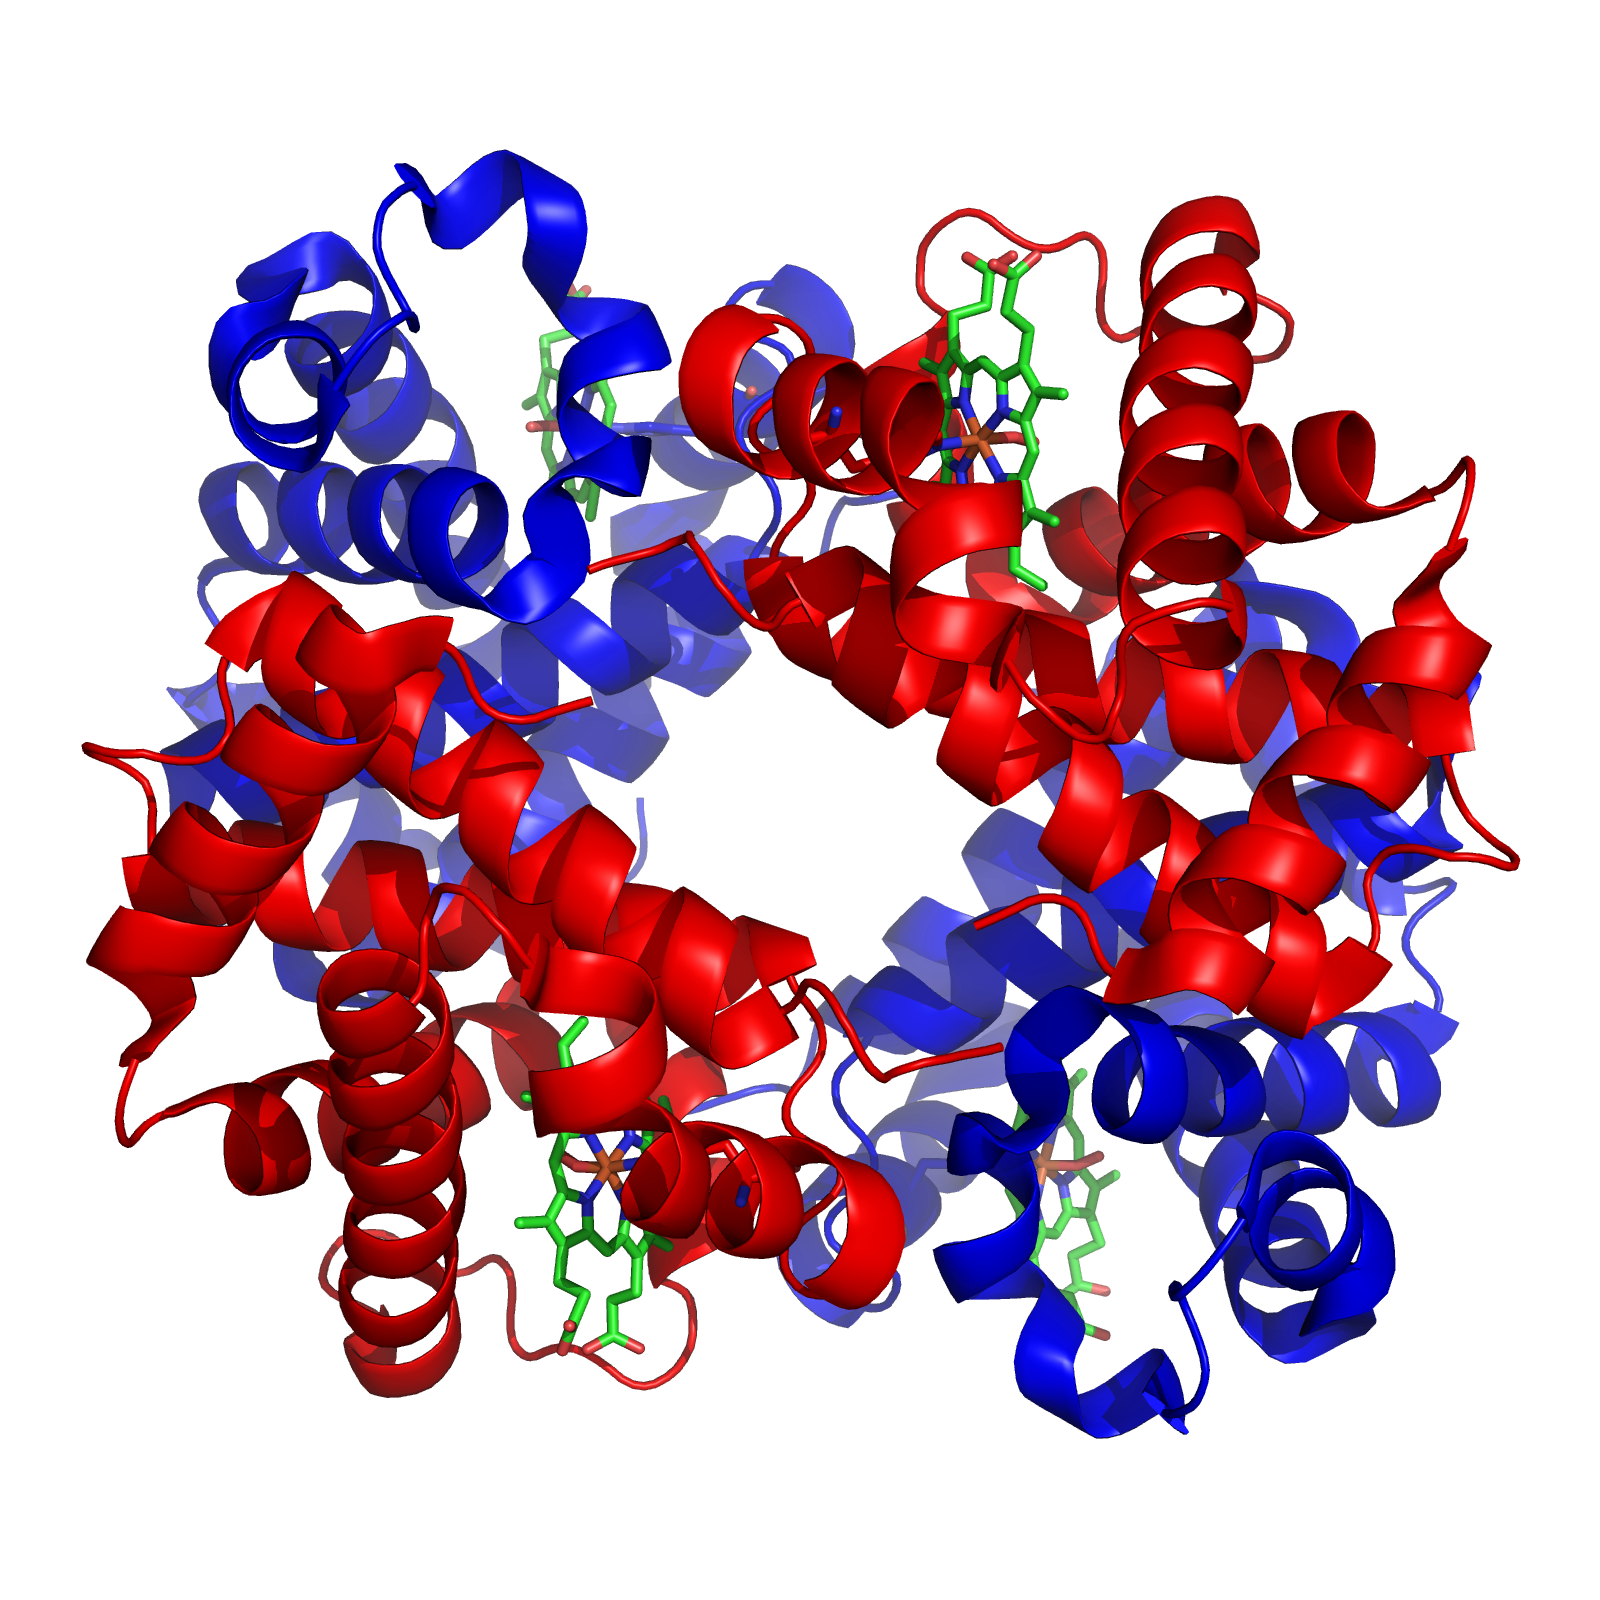
\includegraphics[width=\linewidth]{./dipterv1_figures/hemoglobin.png}
    \caption{Protein folding (Hemoglobin)}
  \end{subfigure}
\end{figure}

\end{frame}


\begin{frame}{"Protein folding" kvantumos modellje}

\begin{columns}
\begin{column}{0.55\textwidth}
\vspace{-0.3cm}
\begin{itemize}
    \item \textbf{Protein}:
    \begin{itemize}
        \item Aminosavakból alkotott lánc.
        \begin{itemize}
          \item \color{red} Piros = Hidrofób (''vízkerülő'').
          \item \color{blue} Kék = Poláris (''vízszerető'').
        \end{itemize}
        \item Hajtogatás: 3D kockarács pontjain.
        \item Cél: Minimális energiájú elhelyezés (NP-nehéz).
    \end{itemize}
    \item \textbf{Kódolás}:
    \begin{itemize}
        \item Origóból, lépésenként \\$6$ irány $=$ $6$ kvantumbit (qubit).
    \end{itemize}
    \item \textbf{Orákulum}: 
    \begin{itemize}
        \item Energiaviszonyok lepontozása.
    \end{itemize}
\end{itemize}
\end{column}
\begin{column}{0.45\textwidth}
\vspace{-0.2cm}
\begin{figure}[H]
\center
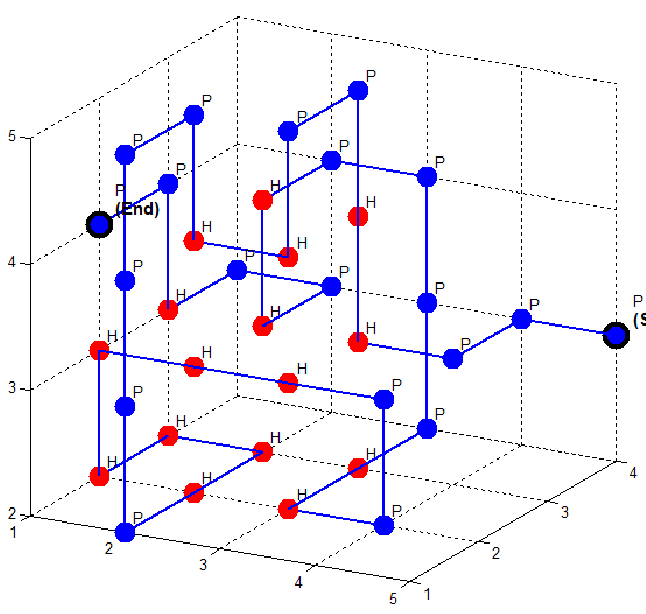
\includegraphics[width=\textwidth]{./tdk_2022_figures/Protein-folds-with-length-36-amino-acids-18-contacts.png}
\caption{Egy összehajtogatott protein.\footnotemark}
\end{figure}
\end{column}
\end{columns}

\footnotetext[1]{\scriptsize Forrás: Traykov et al. (2018). Protein Folding in 3D Lattice HP Model Using Heuristic Algorithm.}

\end{frame}

\begin{frame}{Kvantumalgoritmusok a megoldáshoz}
\begin{itemize}
    \item \textbf{Grover-algoritmus}
    \begin{itemize}
        \item Strukturálatlan keresés.
        \item \textbf{Klasszikusan} $O(N)$: minden lehetséges megoldás végignézése.
        \item \textbf{Kvantumosan} $O(\sqrt{N})$: ''kvantum párhuzamosság'' kihasználása. 
    \end{itemize}
    \item \textbf{Kvantumséták}
    \begin{itemize}
        \item Strukturált keresés.
        \item \textbf{Gráf}:
        \begin{itemize}
            \item Csúcsai: lehetséges hajtogatások.
            \item Élei: apró transzformációk.
        \end{itemize}
    \end{itemize}
   \item $\rightarrow$ Kettő kombinálása.
\end{itemize}
\end{frame}

\begin{frame}{Kvantumséták szimulációja (128 csúcsú kör)}
\begin{figure}[H]
  \centering
  \includegraphics[width=0.30\linewidth]{./cikk_figures/results/cycle_long/classical.eps}
  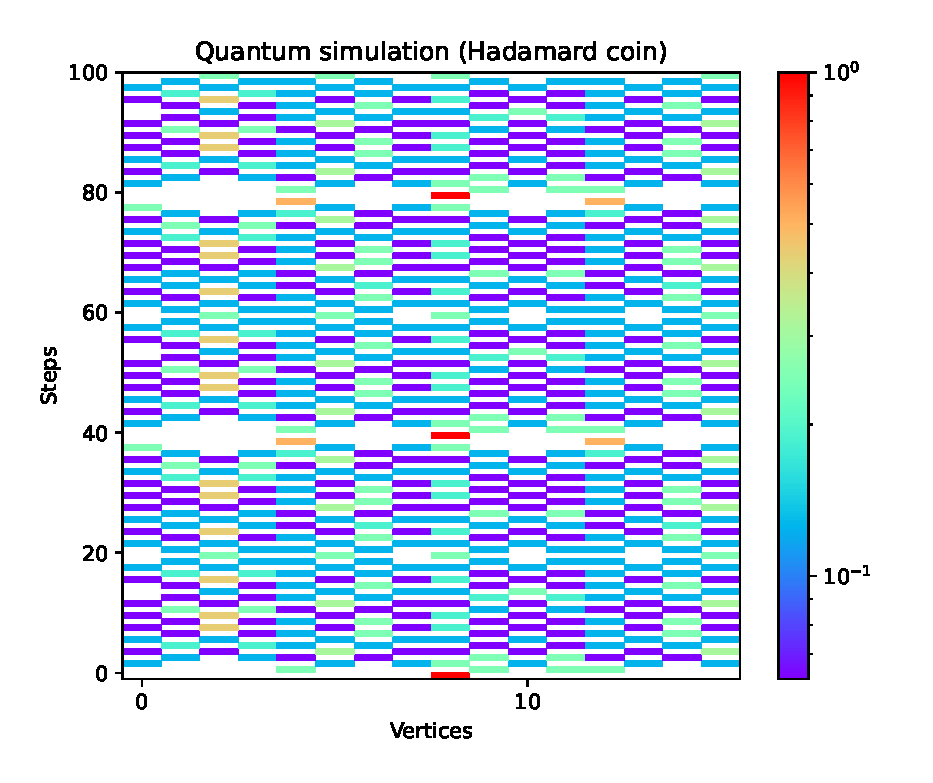
\includegraphics[width=0.30\linewidth]{./cikk_figures/results/cycle_long/hadamard.eps}
\end{figure}
\end{frame}

\begin{frame}{Kvantumséták szimulációja (4D, 16 csúcsú hiperkocka)}

\begin{columns}
\begin{column}{0.20\linewidth}
\end{column}
\begin{column}{0.30\linewidth}
\begin{center}
\includegraphics[width=\linewidth]{./cikk_figures/results/hypercube/classical.eps}
\newline
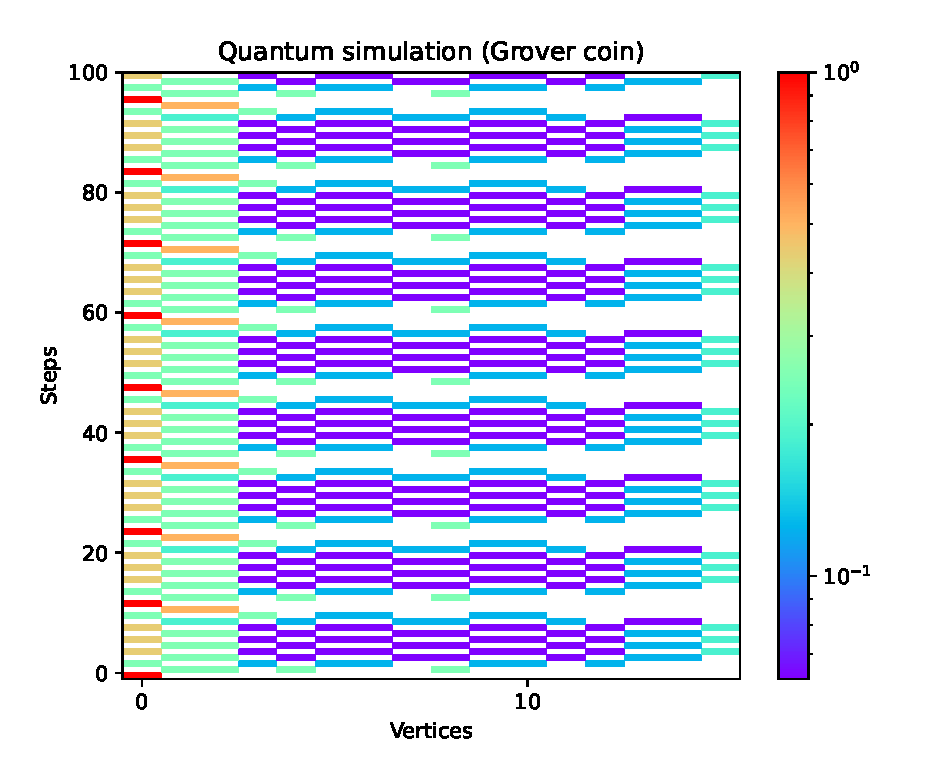
\includegraphics[width=\linewidth]{./cikk_figures/results/hypercube/grover.eps}
\end{center}
\end{column}
\begin{column}{0.30\linewidth}
\begin{center}
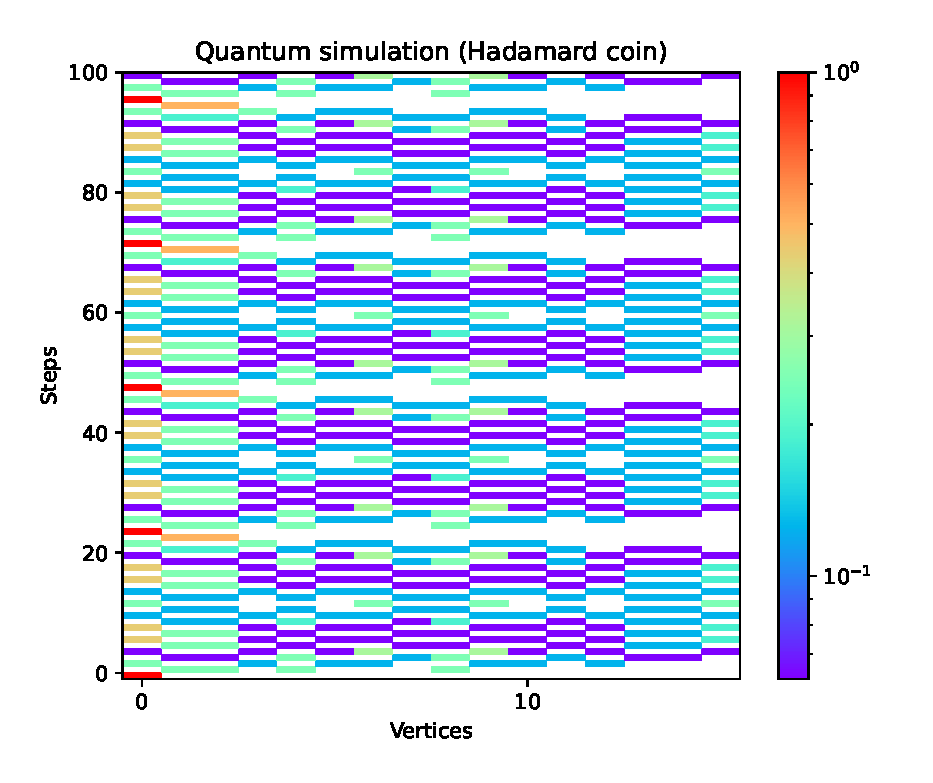
\includegraphics[width=\linewidth]{./cikk_figures/results/hypercube/hadamard.eps}
\newline
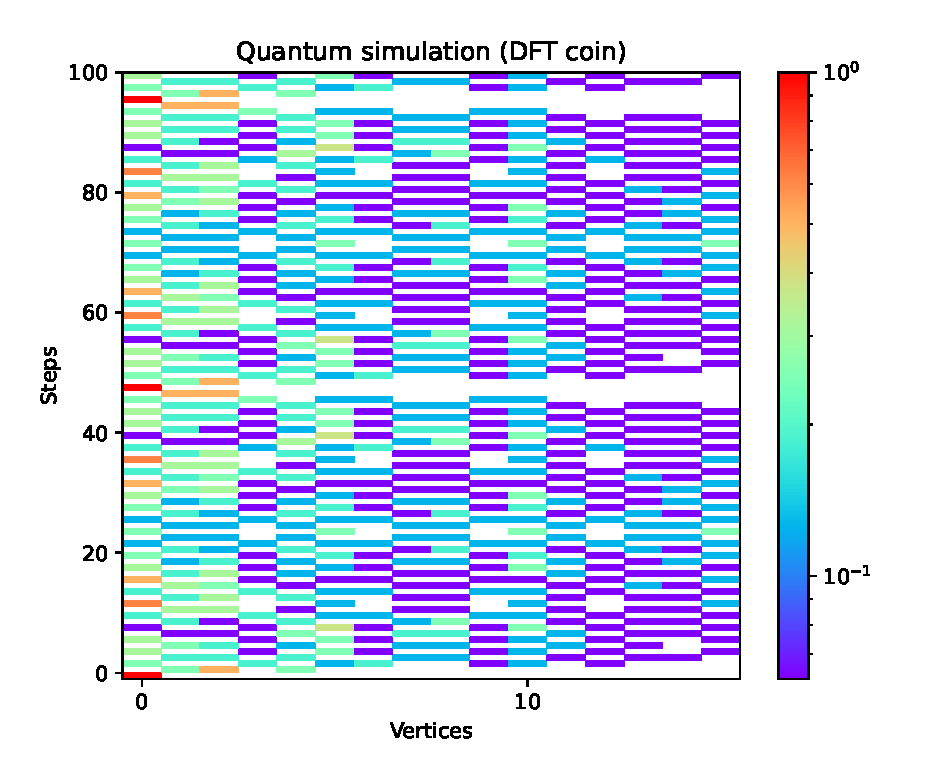
\includegraphics[width=\linewidth]{./cikk_figures/results/hypercube/dft.eps}
\end{center}
\end{column}
\begin{column}{0.20\linewidth}
\end{column}
\end{columns}



\end{frame}

\begin{frame}{Memóriafelhasználás optimalizálása kvantumalgoritmusok szimulációjában}

\end{frame}

\begin{frame}{Zárszó}

\begin{center}
\begin{LARGE}
Köszönöm a figyelmet!
\end{LARGE}
\end{center}

\begin{itemize}
\item \textbf{Forráskódok} (MIT licensz)
\begin{itemize}
\item Kvantumséták: \href{https://github.com/nemkin/quantum-walk}{\color{blue}https://github.com/nemkin/quantum-walk}
\item Memóriaoptimalizálás: \href{https://github.com/nemkin/qmem}{\color{blue}https://github.com/nemkin/qmem}
\end{itemize}
\end{itemize}
\end{frame}

\begin{frame}{Bíráló kérdései - 1.}

A szerző említi (30. oldal), hogy ha egy gráf szomszédsági mátrixa felírható permutációk összegeként, akkor létezik rá kvantumbolyongás. Tudna mondani egy vagy több feltételt vagy példát, hogy ez milyen mátrixokra/gráfokra teljesül?

\begin{itemize}
  \item 
\end{itemize}

\end{frame}

\begin{frame}{Bíráló kérdései - 2.}

Az 5.6. ábrán a következők vannak ábrázolva: ,,Quantum [...] hitting and mixing times''. Mi ennek a két fogalomnak a definíciója? (Nem találtam a dolgozatban.)

\begin{itemize}
  \item 
\end{itemize}

\end{frame}

\end{document}